
\documentclass[border=10pt, 12pt]{standalone}
\usepackage[svgnames]{xcolor}
\usepackage{amsmath}
\usepackage{pgfplots}
\pgfplotsset{compat=newest}
\usepackage[sfdefault]{FiraSans}
\usepackage{FiraMono}
\renewcommand*\familydefault{\sfdefault}
\begin{document}
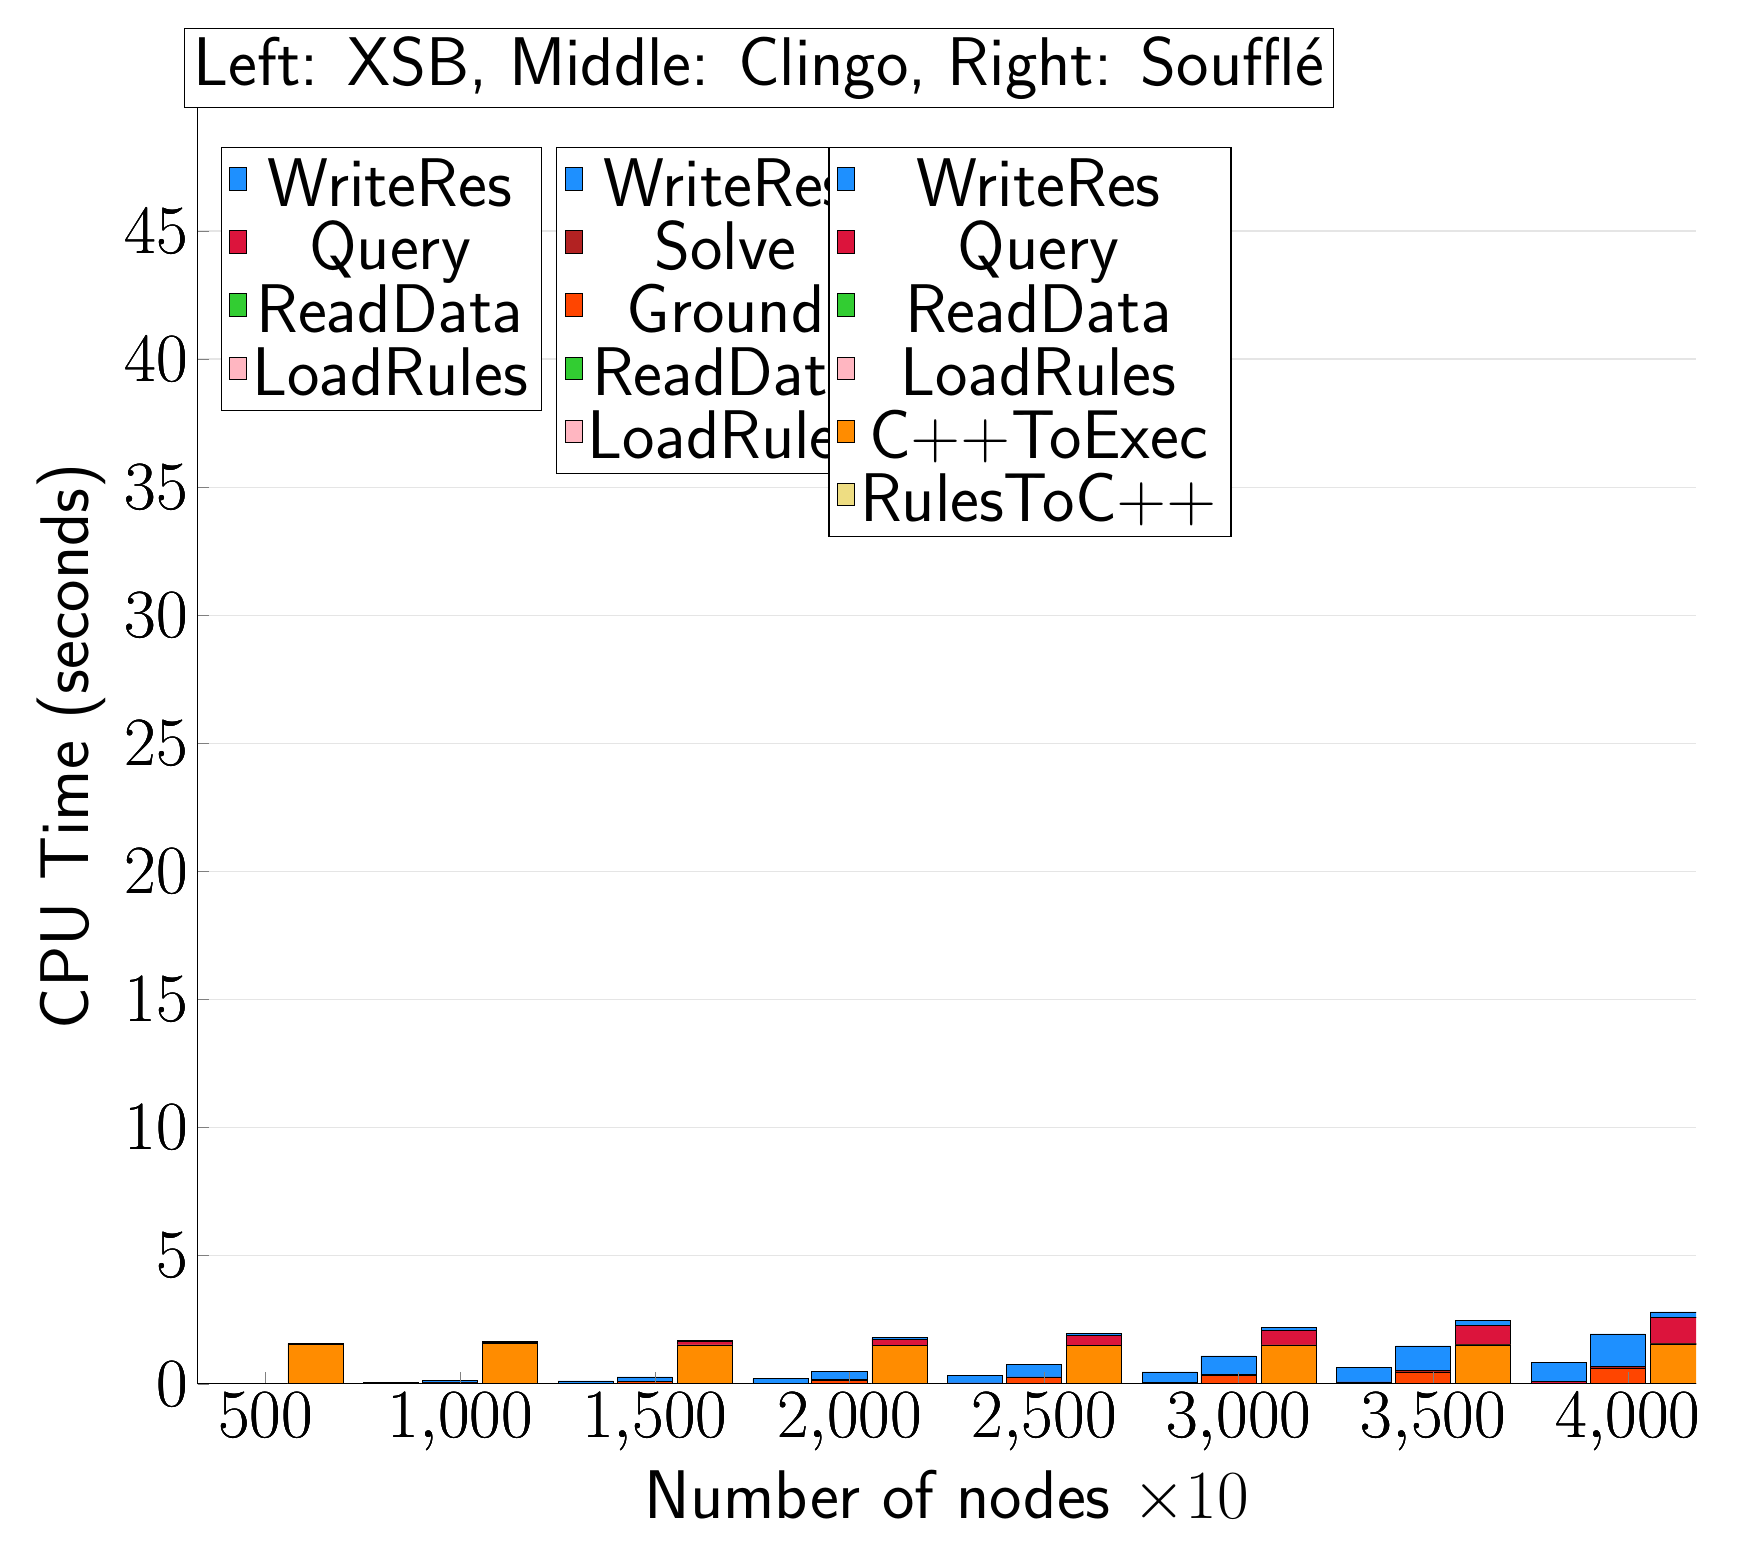
\begin{tikzpicture}
	\begin{axis}[bar shift=-25pt,
			ybar stacked,
			width=1.7\textwidth,
			bar width=0.7cm,
			ymajorgrids, tick align=inside,
			major grid style={draw=gray!20},
			xtick=data,
			ymin=0, ymax=49.78293,
			axis x line*=bottom,
			axis y line*=left,
			enlarge x limits=0.05,
			legend style={
					at={(0.23, 0.97)},
					anchor=north east,
					legend columns=1,
					font=\Huge,
				},
			ylabel={CPU Time (seconds)},
			xlabel={Number of nodes $\times 10$},
			label style={font=\Huge},
			tick label style={font=\Huge},
		]
		\addlegendimage{fill=DodgerBlue, draw=black, line width=0.2pt}
		\addlegendentry{WriteRes}
		\addlegendimage{fill=Crimson, draw=black, line width=0.2pt}
		\addlegendentry{Query}
		\addlegendimage{fill=LimeGreen, draw=black, line width=0.2pt}
		\addlegendentry{ReadData}
		\addlegendimage{fill=LightPink, draw=black, line width=0.2pt}
		\addlegendentry{LoadRules}
		\addplot +[fill=LightPink, draw=black, line width=0.2pt] coordinates {
				(500, 0.0006144000000000004)
				(1000, 0.0006170000000000001)
				(1500, 0.0006036000000000001)
				(2000, 0.0006014000000000002)
				(2500, 0.0006100000000000003)
				(3000, 0.0006083000000000001)
				(3500, 0.0006330999999999999)
				(4000, 0.0006348999999999995)
			};
		\addplot +[fill=LimeGreen, draw=black, line width=0.2pt] coordinates {
				(500, 0.0005751999999999997)
				(1000, 0.001001399999999999)
				(1500, 0.0014525)
				(2000, 0.0019239000000000003)
				(2500, 0.0023976)
				(3000, 0.0028595)
				(3500, 0.0032928)
				(4000, 0.0037789000000000004)
			};
		\addplot +[fill=Crimson, draw=black, line width=0.2pt] coordinates {
				(500, 0.0013463999999999998)
				(1000, 0.005301599999999999)
				(1500, 0.0119086)
				(2000, 0.0221653)
				(2500, 0.0338746)
				(3000, 0.050072799999999994)
				(3500, 0.0680577)
				(4000, 0.0915405)
			};
		\addplot +[fill=DodgerBlue, draw=black, line width=0.2pt] coordinates {
				(500, 0.011429)
				(1000, 0.046037499999999995)
				(1500, 0.10270350000000002)
				(2000, 0.18078100000000003)
				(2500, 0.2857507)
				(3000, 0.4086659)
				(3500, 0.5595814000000001)
				(4000, 0.7277069)
			};
	\end{axis}

	\begin{axis}[bar shift=-3.7pt,
			ybar stacked,
			width=1.7\textwidth,
			bar width=0.7cm,
			ymajorgrids, tick align=inside,
			major grid style={draw=none},
			xtick=data,
			ymin=0, ymax=49.78293,
			axis x line*=none,
			axis y line*=none,
			enlarge x limits=0.05,
			legend style={
					at={(0.454, 0.97)},
					anchor=north east,
					legend columns=1,
					font=\Huge,
				},
			label style={font=\Huge},
			tick label style={font=\Huge},
		]
		\addlegendimage{fill=DodgerBlue, draw=black, line width=0.2pt}
		\addlegendentry{WriteRes}
		\addlegendimage{fill=FireBrick, draw=black, line width=0.2pt}
		\addlegendentry{Solve}
		\addlegendimage{fill=OrangeRed, draw=black, line width=0.2pt}
		\addlegendentry{Ground}
		\addlegendimage{fill=LimeGreen, draw=black, line width=0.2pt}
		\addlegendentry{ReadData}
		\addlegendimage{fill=LightPink, draw=black, line width=0.2pt}
		\addlegendentry{LoadRules}
		\addplot +[fill=LightPink, draw=black, line width=0.2pt] coordinates {
				(500, 0.0)
				(1000, 0.0)
				(1500, 0.0)
				(2000, 0.0)
				(2500, 0.0)
				(3000, 0.0)
				(3500, 0.0)
				(4000, 0.0)
			};
		\addplot +[fill=LimeGreen, draw=black, line width=0.2pt] coordinates {
				(500, 0.0)
				(1000, 0.0009999999999999998)
				(1500, 0.0)
				(2000, 0.009999999999999997)
				(2500, 0.009999999999999997)
				(3000, 0.009999999999999997)
				(3500, 0.009999999999999997)
				(4000, 0.009999999999999997)
			};
		\addplot +[fill=OrangeRed, draw=black, line width=0.2pt] coordinates {
				(500, 0.009999999999999997)
				(1000, 0.038999999999999986)
				(1500, 0.07999999999999999)
				(2000, 0.13199999999999998)
				(2500, 0.229)
				(3000, 0.33)
				(3500, 0.45200000000000007)
				(4000, 0.602)
			};
		\addplot +[fill=FireBrick, draw=black, line width=0.2pt] coordinates {
				(500, 0.0)
				(1000, 0.0010000000000000009)
				(1500, 0.009999999999999995)
				(2000, 0.01899999999999999)
				(2500, 0.03100000000000002)
				(3000, 0.04100000000000003)
				(3500, 0.06500000000000004)
				(4000, 0.07699999999999999)
			};
		\addplot +[fill=DodgerBlue, draw=black, line width=0.2pt] coordinates {
				(500, 0.020000000000000007)
				(1000, 0.08399999999999999)
				(1500, 0.17799999999999996)
				(2000, 0.32100000000000006)
				(2500, 0.48200000000000004)
				(3000, 0.7049999999999998)
				(3500, 0.9570000000000002)
				(4000, 1.261)
			};
	\end{axis}

	\begin{axis}[bar shift=18pt,
			ybar stacked,
			width=1.7\textwidth,
			bar width=0.7cm,
			ymajorgrids, tick align=inside,
			major grid style={draw=none},
			xtick=data,
			ymin=0, ymax=49.78293,
			axis x line*=none,
			axis y line*=none,
			enlarge x limits=0.05,
			legend style={
					at={(0.69, 0.97)},
					anchor=north east,
					legend columns=1,
					font=\Huge,
				},
			label style={font=\Huge},
			tick label style={font=\Huge},
		]
		\addlegendimage{fill=DodgerBlue, draw=black, line width=0.2pt}
		\addlegendentry{WriteRes}
		\addlegendimage{fill=Crimson, draw=black, line width=0.2pt}
		\addlegendentry{Query}
		\addlegendimage{fill=LimeGreen, draw=black, line width=0.2pt}
		\addlegendentry{ReadData}
		\addlegendimage{fill=LightPink, draw=black, line width=0.2pt}
		\addlegendentry{LoadRules}
		\addlegendimage{fill=DarkOrange, draw=black, line width=0.2pt}
		\addlegendentry{C++ToExec}
		\addlegendimage{fill=LightGoldenrod, draw=black, line width=0.2pt}
		\addlegendentry{RulesToC++}
		\addplot +[fill=LightGoldenrod, draw=black, line width=0.2pt] coordinates {
				(500, 0.030000000000000006)
				(1000, 0.030000000000000006)
				(1500, 0.030000000000000006)
				(2000, 0.030000000000000006)
				(2500, 0.030000000000000006)
				(3000, 0.030000000000000006)
				(3500, 0.030000000000000006)
				(4000, 0.030000000000000006)
			};
		\addplot +[fill=DarkOrange, draw=black, line width=0.2pt] coordinates {
				(500, 1.522)
				(1000, 1.5400000000000003)
				(1500, 1.4850000000000003)
				(2000, 1.4700000000000002)
				(2500, 1.473)
				(3000, 1.483)
				(3500, 1.4889999999999999)
				(4000, 1.525)
			};
		\addplot +[fill=LightPink, draw=black, line width=0.2pt] coordinates {
				(500, 8.209999999999999e-05)
				(1000, 7.439999999999999e-05)
				(1500, 0.00010890000000000002)
				(2000, 0.00010740000000000001)
				(2500, 0.00011150000000000001)
				(3000, 9.92e-05)
				(3500, 8.58e-05)
				(4000, 0.00010250000000000001)
			};
		\addplot +[fill=LimeGreen, draw=black, line width=0.2pt] coordinates {
				(500, 0.0011086)
				(1000, 0.0019181000000000003)
				(1500, 0.0035159999999999996)
				(2000, 0.004493200000000001)
				(2500, 0.005503900000000001)
				(3000, 0.006535400000000001)
				(3500, 0.007031999999999999)
				(4000, 0.0080124)
			};
		\addplot +[fill=Crimson, draw=black, line width=0.2pt] coordinates {
				(500, 0.0148894)
				(1000, 0.058338999999999995)
				(1500, 0.13507059999999999)
				(2000, 0.23820510000000006)
				(2500, 0.37549179999999993)
				(3000, 0.5541748)
				(3500, 0.7649524000000001)
				(4000, 1.018127)
			};
		\addplot +[fill=DodgerBlue, draw=black, line width=0.2pt] coordinates {
				(500, 0.004368199999999999)
				(1000, 0.014265799999999999)
				(1500, 0.031566500000000004)
				(2000, 0.0564145)
				(2500, 0.08798500000000001)
				(3000, 0.1261758)
				(3500, 0.17266189999999998)
				(4000, 0.22527880000000003)
			};
	\end{axis}


	\node[anchor=south, draw, fill=white] at (rel axis cs:0.42,1) {\Huge Left: XSB, Middle: Clingo, Right: Soufflé};
\end{tikzpicture}
\end{document}
